%%%%%%%%%%%%%%%%%%%%%%%%%%%%%%%%%%%%%%%%%%%%%%%%%%%%%%%%%%%%%%%%%%%%%%%%%%%%%%%
\documentclass[hyperref={pdfpagelabels=false},compress,table]{beamer} % 在Mac下无法编译
% \documentclass[compress,table]{beamer} % 在Mac下使用
% package for font
\usepackage{fontspec}
\defaultfontfeatures{Mapping=tex-text}  %%如果没有它,会有一些 tex 特殊字符无法正常使用,比如连字符。
\usepackage{xunicode,xltxtra}
\usepackage[BoldFont,SlantFont,CJKnumber,CJKchecksingle]{xeCJK}  % \CJKnumber{12345}: 一万二千三百四十五
\usepackage{CJKfntef}  %%实现对汉字加点、下划线等。
\usepackage{pifont}  % \ding{}
% package for math
\usepackage{amsfonts}

% package for graphics
\usepackage[americaninductors,europeanresistors]{circuitikz}
\usepackage{tikz}
\usetikzlibrary{plotmarks}  % placements=positioning
\usepackage{graphicx}  % \includegraphics[]{}
\usepackage{subfigure}  %%图形或表格并排排列
% package for table
\usepackage{colortbl,dcolumn}  %% 彩色表格
\usepackage{multirow}
\usepackage{multicol}
\usepackage{booktabs}
% package for code
\usepackage{fancyvrb}
\usepackage{listings}

% \usepackage{animate}
% \usepackage{movie15}

%%%%%
% setting for beamer
\usetheme{default} % Madrid(常用), Copenhagen, AnnArbor, boxes(白色), Frankfurt,Berkeley
\useoutertheme[subsection=true]{miniframes} % 使用Berkeley时注释本行
\usecolortheme{sidebartab}
\usefonttheme{serif}  %%英文使用衬线字体
% \setbeamertemplate{background canvas}[vertical
% shading][bottom=white,top=structure.fg!7] %%背景色,上25%的蓝,过渡到下白。
\setbeamertemplate{theorems}[numbered]
\setbeamertemplate{navigation symbols}{}  %% 去掉页面下方默认的导航条
\setbeamercovered{transparent}  %设置 beamer 覆盖效果

% 设置标题title背景色
% \setbeamercolor{title}{fg=black, bg=lightgray!60!white}
\setbeamercolor{title}{fg=white, bg=black!70!white}

% 设置每页小LOGO
\pgfdeclareimage[width=1cm]{ouc}{figures/static/ouc.pdf}
\logo{\pgfuseimage{ouc}{\vspace{-20pt}}}

% setting for font
%%\setCJKmainfont{Adobe Kaiti Std}
\setCJKmainfont{SimSun} 
%% \setCJKmainfont{FangSong_GB2312} 
%% \setmainfont{Apple Garamond}  %%苹果字体没有SmallCaps
\setCJKmainfont{SimSun} 
%FUNNY%\setCJKmainfont{DFPShaoNvW5-GB}  %%华康少女文字W5(P)
%FUNNY%\setCJKmainfont{FZJingLeiS-R-GB}  %%方正静蕾体
%FUNNY%\setmainfont{Purisa}
%\setsansfont[Mapping=tex-text]{Adobe Song Std}
     %如果装了Adobe Acrobat,可在font.conf中配置Adobe字体的路径以使用其中文字体。
     %也可直接使用系统中的中文字体如SimSun、SimHei、微软雅黑等。
     %原来beamer用的字体是sans family;注意Mapping的大小写,不能写错。
     %设置字体时也可以直接用字体名,以下三种方式等同:
     %\setromanfont[BoldFont={黑体}]{宋体}
     %\setromanfont[BoldFont={SimHei}]{SimSun}
     %\setromanfont[BoldFont={"[simhei.ttf]"}]{"[simsun.ttc]"}
% setting for graphics
\graphicspath{{figures/}}  %%图片路径
\renewcommand\figurename{图}

% setting for pdf
\hypersetup{% pdfpagemode=FullScreen,%
            pdfauthor={Xiaodong Wang},%
            pdftitle={Title},%
            CJKbookmarks=true,%
            bookmarksnumbered=true,%
            bookmarksopen=false,%
            plainpages=false,%
            colorlinks=true,%
            citecolor=green,%
            filecolor=magenta,%
            linkcolor=blue,%red(default)
            urlcolor=cyan}

% setting for fontspec
\XeTeXlinebreaklocale "zh"  %%表示用中文的断行
\XeTeXlinebreakskip = 0pt plus 1pt minus 0.1pt  %%多一点调整的空间
%%%%%

% font setting by xeCJK
\setCJKfamilyfont{NSimSun}{NSimSun}
\newcommand{\song}{\CJKfamily{NSimSun}}
%%%\setCJKfamilyfont{AdobeSongStd}{Adobe Song Std}
%%%\newcommand{\AdobeSong}{\CJKfamily{AdobeSongStd}}
\setCJKfamilyfont{FangSong}{FangSong_GB2312}
\newcommand{\fang}{\CJKfamily{FangSong}}
%%%\setCJKfamilyfont{AdobeFangsongStd}{Adobe Fangsong Std}
%%%\newcommand{\AdobeFang}{\CJKfamily{AdobeFangsongStd}}
\setCJKfamilyfont{SimHei}{SimHei}
\newcommand{\hei}{\CJKfamily{SimHei}}
%%%\setCJKfamilyfont{AdobeHeitiStd}{Adobe Heiti Std}
%%%\newcommand{\AdobeHei}{\CJKfamily{AdobeHeitiStd}}
\setCJKfamilyfont{KaiTi}{KaiTi}
\newcommand{\kai}{\CJKfamily{KaiTi}}
%%%\setCJKfamilyfont{AdobeKaitiStd}{Adobe Kaiti Std}
\newcommand{\AdobeKai}{\CJKfamily{AdobeKaitiStd}}
\setCJKfamilyfont{LiSu}{LiSu}
\newcommand{\li}{\CJKfamily{LiSu}}
\setCJKfamilyfont{YouYuan}{YouYuan}
\newcommand{\you}{\CJKfamily{YouYuan}}
\setCJKfamilyfont{FZJingLei}{FZJingLeiS-R-GB}
\newcommand{\jinglei}{\CJKfamily{FZJingLei}}
\setCJKfamilyfont{MSYH}{Microsoft YaHei}
\newcommand{\msyh}{\CJKfamily{MSYH}}

% 自定义颜色
\def\Red{\color{red}}
\def\Green{\color{green}}
\def\Blue{\color{blue}}
\def\Mage{\color{magenta}}
\def\Cyan{\color{cyan}}
\def\Brown{\color{brown}}
\def\White{\color{white}}
\def\Black{\color{black}}

\lstnewenvironment{xmlCode}[1][]{% for Java
  \lstset{
    basicstyle=\tiny\ttfamily,%
    columns=flexible,%
    framexleftmargin=.7mm, %
    % frame=shadowbox,%
    % rulesepcolor=\color{cyan},%
     frame=single,%
    backgroundcolor=\color{white},%
    xleftmargin=4\fboxsep,%
    xrightmargin=4\fboxsep,%
    numbers=left,numberstyle=\tiny,%
    numberblanklines=false,numbersep=7pt,%
    language=xml, %
    }\lstset{#1}}{}

\lstnewenvironment{javaCode}[1][]{% for Java
  \lstset{
    basicstyle=\tiny\ttfamily,%
    columns=flexible,%
    framexleftmargin=.7mm, %
    frame=shadowbox,%
    rulesepcolor=\color{cyan},%
    % frame=single,%
    backgroundcolor=\color{white},%
    xleftmargin=4\fboxsep,%
    xrightmargin=4\fboxsep,%
    numbers=left,numberstyle=\tiny,%
    numberblanklines=false,numbersep=7pt,%
    language=Java, %
    }\lstset{#1}}{}

\lstnewenvironment{shCode}[1][]{% for Java
  \lstset{
    basicstyle=\scriptsize\ttfamily,%
    columns=flexible,%
    framexleftmargin=.7mm, %
    frame=shadowbox,%
    rulesepcolor=\color{brown},%
    % frame=single,%
    backgroundcolor=\color{white},%
    xleftmargin=4\fboxsep,%
    xrightmargin=4\fboxsep,%
    numbers=left,numberstyle=\tiny,%
    numberblanklines=false,numbersep=7pt,%
    language=sh, %
    }\lstset{#1}}{}

\newcommand\ask[1]{\vskip 4bp \tikz \node[rectangle,rounded corners,minimum size=6mm,
  fill=white,]{\Cyan \includegraphics[height=1.5cm]{question} \Large \msyh #1};}

\newcommand\wxd[1]{\vskip 4bp \tikz \node[rectangle,minimum size=6mm,
  fill=blue!60!white,]{\White \ding{118} \msyh #1};}

\newcommand\xyy[1]{\vskip 2bp \tikz \node[rectangle,minimum size=3mm,
  fill=black!80!white,]{\White \msyh\scriptsize #1};}

\newcommand\homework[1]{\vskip 2bp \tikz \node[rectangle,minimum size=3mm,
  fill=red!80!white,]{\White \ding{45} \msyh\scriptsize 课后小作业 } ; {\kai\small #1}} 

\newcommand\cxf[1]{\vskip 4bp \tikz \node[rectangle,rounded corners,minimum size=6mm,
  fill=purple!60!white,]{\White \ding{42} \msyh #1};}

\newcommand\tta[1]{\vskip 4bp \tikz \node[rectangle,minimum size=6mm,
  fill=blue!60!white,]{\White \ding{118} \msyh #1};}

\newcommand\ttb[1]{\vskip 4bp \tikz \node[rectangle,rounded corners,minimum size=6mm,
  fill=purple!60!white,]{\White \ding{42} \msyh #1};}

\newcommand\ttc[1]{\vskip 2bp \tikz \node[rectangle,minimum size=3mm,
  fill=black!80!white,]{\White \msyh\scriptsize #1};}

\newcommand\notice[1]{\vskip 4bp \tikz \node[rectangle,rounded corners,minimum size=6mm,
  fill=red!80!white,]{\White \scriptsize \ding{42} \msyh #1};}

\newcommand\samp[1]{\vskip 2bp \tikz \node[rectangle,minimum size=3mm,
  fill=white!100!white,]{\Mage\msyh \small CODE \ding{231} \Black #1};\vskip -8bp}

\newcommand\codeset[1]{\vskip 2bp \tikz \node[rectangle,minimum size=3mm,
  fill=white!100!white,]{\Mage\msyh \small 课程配套代码 \ding{231} \Black #1};\vskip -8bp}

\newcommand\pptlink[2]{\vskip 4bp \tikz \node[rectangle,rounded corners,minimum size=6mm,
  fill=blue!70!white,]{\href{run:#1}{\White \scriptsize \msyh 动画演示 #2}};}



\setbeamerfont{frametitle}{series=\msyh} % 修改Beamer标题字体

\makeatletter
\newcommand{\Extend}[5]{\ext@arrow 0099{\arrowfill@#1#2#3}{#4}{#5}}
\makeatother


%%%%%%%%%%%%%%%%%%%%%%%%%%%%%%%%%%%%%%%%%%%%%%%%%%%%%%%%%%%%%%%%%%%%%%%%%%%%%%%
% \titlepage
\title[KevinW@OUC]{\hei {\huge Java 应用与开发}\\  
  高级I/O编程}
\author[王晓东]{王晓东\\
  \href{mailto:wangxiaodong@ouc.edu.cn}{\footnotesize wangxiaodong@ouc.edu.cn}}
\institute[中国海洋大学]{\small 中国海洋大学}
\date{\today}
\titlegraphic{\vspace{-6em}
\includegraphics[height=6cm]{static/ouc.pdf}\vspace{-6em}}
%%%%%
\begin{document}
%% Delete this, if you do not want the table of contents to pop up at
%% the beginning of each subsection:
\AtBeginSection[]{                              % 在每个Section前都会加入的Frame
  \frame<handout:0>{
    \frametitle{\textbf{\hei 接下来…}}
    \tableofcontents[currentsection]
  }
}  %

\AtBeginSubsection[]                            % 在每个子段落之前
{
  \frame<handout:0>                             % handout:0 表示只在手稿中出现
  {
    \frametitle{\textit{\hei 接下来…}}\small
    \tableofcontents[current,currentsubsection] % 显示在目录中加亮的当前章节
  }
}
\frame{\titlepage}
%%%%%%%%%%%%%%%%%%%%%%%%%%%%%%%%%%%%%%%%%%%%%%%%%%%%%%%%%%%%%%%%%%%%%%%%%%%%%%%
\begin{frame}
  \frametitle{学习目标}
  \begin{enumerate}
  \item 深入理解Java的I/O原理
  \item 掌握Java基本I/O流类型
  \item 掌握I/O的几种应用编程方式
  \end{enumerate}
\end{frame}
%%%%%%%%%%%%%%%%%%%%%%%%%%%%%%%%%%%%%%%%%%%%%%%%%%%%%%%%%%%%%%%%%%%%%%%%%%%%%%%
\section*{大纲}
\frame{\frametitle{大纲} \tableofcontents }
%%%%%%%%%%%%%%%%%%%%%%%%%%%%%%%%%%%%%%%%%%%%%%%%%%%%%%%%%%%%%%%%%%%%%%%%%%%%%%%

\section{Java I/O原理}

\begin{frame}[fragile] % [fragile]参数使得能够插入代码
\frametitle{Java I/O原理}

\tta{ I/O(Input/Output)基本概念}

\begin{itemize}
\item 数据源(Data Source)
\item 数据宿(Data Sink)
\item 流(Stream)\\
  {\kai Java中把不同的数据源与程序间的数据传输都抽象表述为流,java.io包中定义
    了多种I/O流类型实现数据I/O功能。}
\end{itemize}
\end{frame}

\begin{frame}[fragile] % [fragile]参数使得能够插入代码
  \frametitle{Java I/O流的分类}

  \tta{按照数据流动的方向}

  {\hei Java流可分为输入流(Input Stream)和输出流(Output Stream)。}

  \begin{itemize}
  \item 输入流只能从中读取数据,而不能向其写出数据;
  \item 输出流则只能向其写出数据,而不能从中读取数据。
  \item {\Mage (特例 java.io.RandomAccessFile类)}
  \end{itemize}
\end{frame}

\begin{frame}[fragile] % [fragile]参数使得能够插入代码
  \frametitle{Java I/O流的分类}

  \tta{根据数据流所关联的是数据源还是其他数据流}  

  {\hei 可分为节点流(Node Stream)和处理流(Processing Stream)。}

  \begin{itemize}
  \item 节点流直接连接到数据源;
  \item 处理流是对一个已存在的流的连接和封装,通过所封装的流的功能调用
    实现增强的数据读/写功能,处理流并不直接连到数据源。
  \end{itemize}

  \begin{figure}
    \centering
    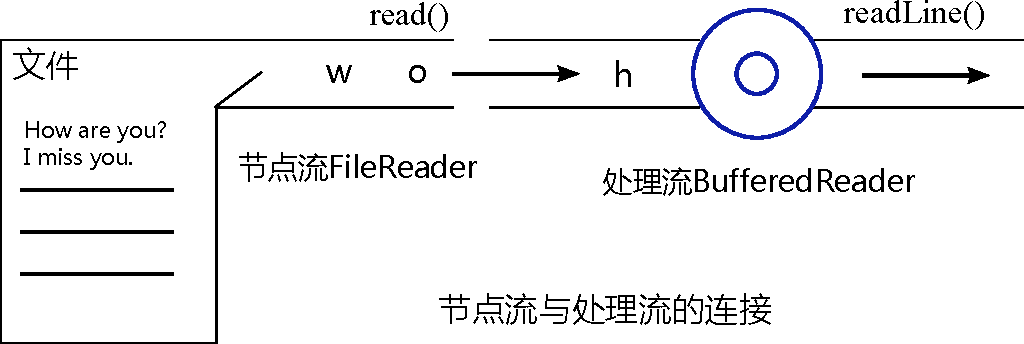
\includegraphics[width=0.7\textwidth]{fig01.pdf}
  \end{figure}
\end{frame}

\begin{frame}[fragile] % [fragile]参数使得能够插入代码
  \frametitle{Java I/O流的分类}

  \tta{按传输数据的“颗粒大小”}

  {\hei 可分为字符流(Character Stream)和字节流(Byte
    Stream)。}

  \begin{itemize}
  \item 字节流以字节为单位传输数据,每次传送一个或多个字节。
  \item 字符流以字符为单位传输数据,每次传送一个或多个字
    符。\footnote{从JDK1.4版本开始,Sun公司引入了新的Java I/O
      API(NIO, New Input/Output),提供面向数据块、异步I/O操作。}
\end{itemize}
  \notice{Java命名惯例}

  凡是以InputStream或OutputStream结尾的类型均为{\hei 字节流},凡是
  以Reader或Writer结尾的均为{\hei 字符流。}
\end{frame}

\section{基础I/O流}

\begin{frame}[fragile] % [fragile]参数使得能够插入代码
\frametitle{InputStream and OutputStream}

\begin{figure}
\centering
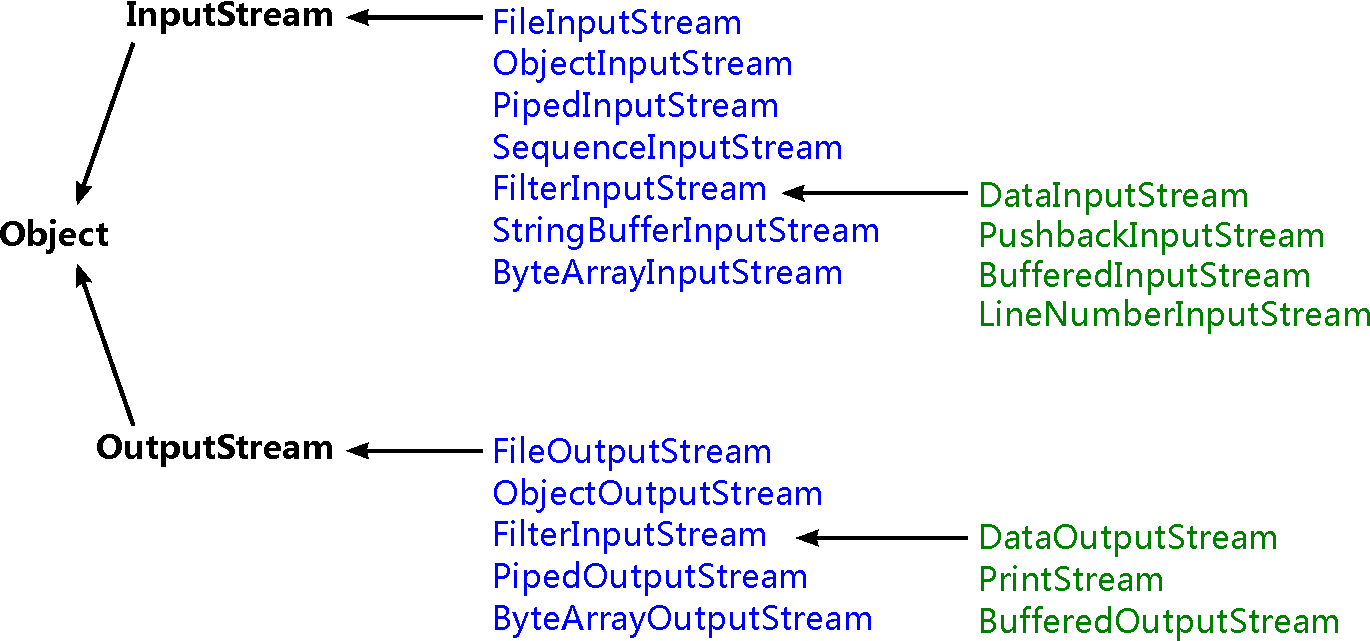
\includegraphics[width=0.85\textwidth]{fig02.pdf}
\end{figure}
\end{frame}

\begin{frame}[fragile] % [fragile]参数使得能够插入代码
\frametitle{InputStream}

抽象类java.io.InputStream是所有字节输入流类型的父类,该类中定义了以字节为单
位读取数据的基本方法,并在其子类中进行了分化和实现。

\xyy{三个基本的read方法}
\begin{itemize}
\item int read()
\item int read(byte[] buffer)
\item int read(byte[] buffer, int offset, int length)
\end{itemize}
\xyy{其它方法}
\begin{itemize}
\item void close()
\item int available()
\item skip(long n)
\item boolean markSupported()
\end{itemize}
\end{frame}

\begin{frame}[fragile] % [fragile]参数使得能够插入代码
\frametitle{OutputStream}

java.io.OutputStream与java.io.InputStream对应,是所有字节输出流类型的抽象父类。

\xyy{三个基本的write方法}
\begin{itemize}
\item void write(int c)
\item void write(byte[] buffer)
\item void write(byte[] buffer, int offset, int length)
\end{itemize}
\xyy{其它方法}
\begin{itemize}
\item void close()
\item void flush()
\end{itemize}
\end{frame}

\begin{frame}[fragile] % [fragile]参数使得能够插入代码
\frametitle{Reader and Writer}

\begin{figure}
\centering
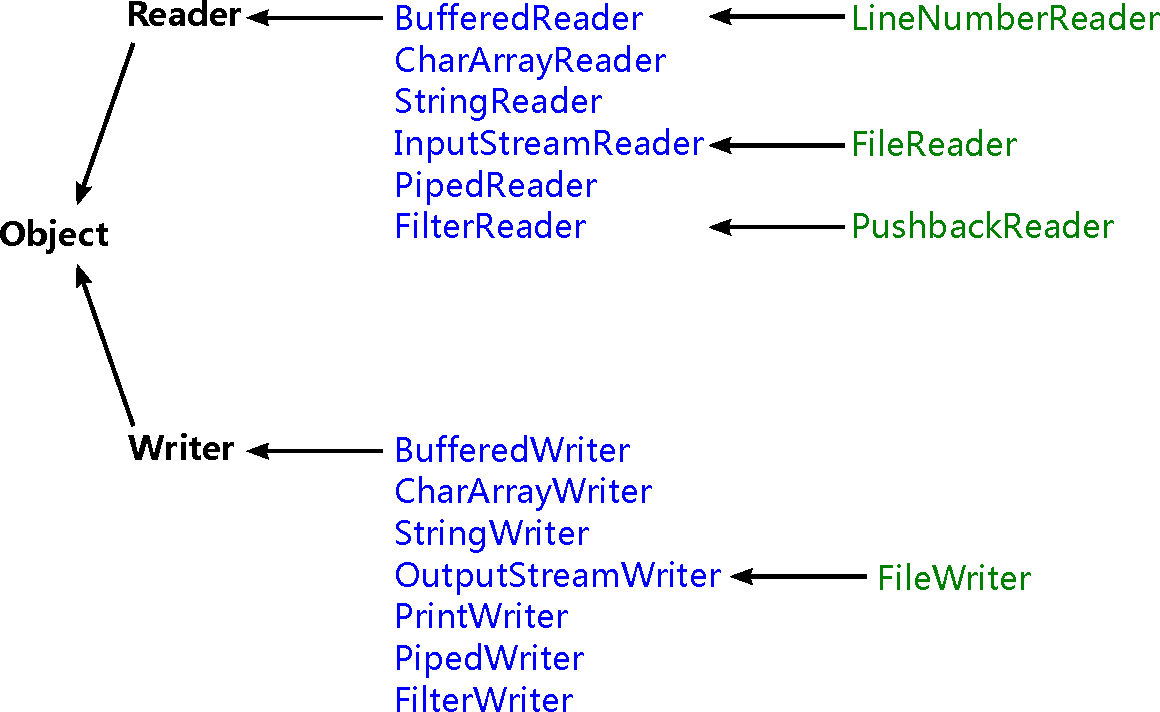
\includegraphics[width=0.85\textwidth]{fig03.pdf}
\end{figure}
\end{frame}

\begin{frame}[fragile] % [fragile]参数使得能够插入代码
\frametitle{Reader}

抽象类java.io.Reader是所有字符输入流类型的父类,其中声明了用于读取字符流的有关方法。
\xyy{三个基本的read方法}
\begin{itemize}
\item int read()
\item int read(char[] cbuf)
\item int read(char[] cbuf, int offset, int length)
\end{itemize}

\xyy{其它方法}
\begin{itemize}
\item void close()
\item boolean ready()
\item skip(long n)
\item boolean markSupported()
\item void mark(int readAheadLimit)
\end{itemize}
\end{frame}

\begin{frame}[fragile] % [fragile]参数使得能够插入代码
\frametitle{Writer}

java.io.Writer与java.io.Reader类对应,是所有字符输出流类型的共同父类。
\xyy{五个基本的write方法}
\begin{itemize}
\item void write(int c)
\item void write(char[] cbuf)
\item void write(char[] cbuf, int offset, int length)
\item void write(String string)
\item void write(String string, int offset, int length)
\end{itemize}
\xyy{其它方法}
\begin{itemize}
\item void close()
\end{itemize}
\end{frame}

\section{常用I/O流类型}

\begin{frame}[fragile] % [fragile]参数使得能够插入代码
\frametitle{FileInputStream/FileOutputStream}
\begin{itemize}
\item FileInputStream用于读取本地文件中字节数据,FileOutputStream用于将字节数据写出到文
  件。
\item FilenputStream不适合获取文本文件中的字符信息,要读取并显示的文件中如果含有双字节字
  符(如中文),则会显示乱码,此时应该采用字符流类型。
\item {\Red \it 可以用于复制任何格式的文件,如文本、音视频以及可执行文件等二进制文件,因为以
    字节为单位进行数据复制时并不对文件内容进行解析。}
\end{itemize}
\samp{Fragment: 使用字节流实现文件复制}
\begin{javaCode}
FileInputStream fis = new FileInputStream("in.txt");
FileOutputStream fos = new FileOutputStream("out.txt");
int read = fis.read();
while (read != -1) {
  fos.write(read);
  read = fis.read();
} 
fis.close();
fos.close();
\end{javaCode}
\end{frame}

\begin{frame}[fragile] % [fragile]参数使得能够插入代码
\frametitle{FileReader/FileWriter}
\begin{itemize}
\item FileReader用于以{\hei 字符}为单位读取文本文件,FileWriter类用于将字符数据写出到文
  本文件。
\item 字符I/O流类型只能处理文本文件,因为二进制文件中保存的字节信息不能正常解析为字符。
\end{itemize}
\samp{Fragment: 使用字符流实现文件复制}
\begin{javaCode}
FileReader fis = new FileReader("in.txt");
// The second arg is boolean append, true for appending, false for covering.
FileWriter fos = new FileWriter("out.txt", true); 
int read = fis.read();
while (read != -1) {
  fos.write(read);
  read = fis.read();
} 
fis.close();
fos.close();
\end{javaCode}
\end{frame}

\begin{frame}[fragile] % [fragile]参数使得能够插入代码
\frametitle{BufferedReader/BufferedWriter}
\begin{itemize}
\item BufferedReader用于缓冲读取字符、字符数组或行,采用缓冲处理能够提高效率,该类所封装
  的字节输入流对象需要在构造方法中指定。
  
  \begin{itemize}
  \item public BufferedReader(Reader in)
  \item public BufferedReader(Reader in, int size) // size of buffer
  \end{itemize}
\item BufferedWriter提供字符的缓冲写出功能,该类的newLine()方法可以写出平台相关的行分隔符
  来标记一行的终止,此分割符由系统属性line.separator确定。
\end{itemize}
\samp{Fragment: 使用字符处理流实现文件复制}
\begin{javaCode}
BufferedReader br = new BufferedReader(new FileReader("in.txt"));
BufferedWriter bw = new BufferedWriter(new FileWriter("out.txt"));
String s = br.readLine();
while (s != null) {
  bw.write(s);
  bw.newLine(); // notice.
  s = br.readLine();
}
\end{javaCode}
\end{frame}

\begin{frame}[fragile] % [fragile]参数使得能够插入代码
\frametitle{Other I/O Classes}
\begin{itemize}
\item InputStreamReader/OutputStreamWriter
\item PrintStream/PrintWriter
\item DataInputStream/DataOutputStream
\item CharArrayReader/CharArrayWriter
\end{itemize}
\end{frame}

\section{I/O应用}



\begin{frame}[fragile] % [fragile]参数使得能够插入代码
\frametitle{属性信息的导入/导出}

如果要永久记录用户自定义的属性,可以采用Properties类的load()/store()方法进行属性的导入/导
出操作,即将属性信息写出到文件中和从文件中读取属性信息到程序。
\samp{SaveProperties.java}
\begin{javaCode}
import java.io.FileWriter;
import java.util.Properties;
public class SaveProperties {
  public static void main(String[] args) {
    try {
      Properties ps = new Properties();
      ps.setProperty("name", "Kevin");
      ps.setProperty("password", "12345");
      FileWriter fw = new FileWriter("props.txt");
      ps.store(fw, "loginfo");
      fw.close();
    } catch (Exception e) {
      e.printStackTrace();
    }
  }
}
\end{javaCode}

\end{frame}

\begin{frame}[fragile] % [fragile]参数使得能够插入代码
\frametitle{属性信息的导入/导出}
\samp{LoadProperties.java}
\begin{javaCode}
import java.io.FileWriter;
import java.util.Properties;
public class LoadProperties {
  public static void main(String[] args) {
    try {
      Properties ps = new Properties();
      FileReader fr = new FileReader("props.txt");
      ps.load(fr);
      fr.close();
      ps.list(System.out);
    } catch (Exception e) {
      e.printStackTrace();
    }
  }
}
\end{javaCode}
\begin{columns}
\column{0.1\textwidth}
\column{0.4\textwidth}
File: props.txt\\
{\tiny
\begin{verbatim}
#loginfo
#Sun Nov 04 21:20:17 CST 2012
password=12345
name=Kevin
\end{verbatim}}
\column{0.4\textwidth}
Stdout \\
{\tiny
\begin{verbatim}
-- listing properties --
password=12345
name=Kevin
\end{verbatim}}
\column{0.1\textwidth}
\end{columns}
\end{frame}




\begin{frame}[fragile] % [fragile]参数使得能够插入代码
\frametitle{对象序列化}

\tta{概念}\\
\small 对象序列化(Object Serialization)是指将对象的状态数据以字节流的形式进行处理,一般
用于实现对象的持久性,即长久保存一个对象的状态并在需要时获取该对象的信息以重新构造一个状
态完全相同的对象。对象序列化可以理解为使用I/O“对象流”类型实现对象读/写操作。

\tta{基本概念}\\
\begin{itemize}\kai\small
\item {\hei 对象的持久性(Object Persistance)} 长久保存一个对象的状态并在需要时获取该对
  象的信息以重新构造一个状态完全相同的对象。
\item {\hei 对象序列化(Object Serialization)} 通过写出对象的状态数据来记录一个对象。
\item {\hei 对象序列化的主要任务} 写出对象的状态信息,并遍历该对象对其他对象的引用,递归
  的序列化所有被引用到的其他对象,从而建立一个完整的序列化流。
\end{itemize}
\end{frame}

\begin{frame}[fragile] % [fragile]参数使得能够插入代码
\frametitle{实现对象序列化}

要序列化一个对象,其所属的类必须实现以下两种接口之一:

\begin{itemize}
\item java.io.Serializable
\item java.io.Externalizable
\end{itemize}

java.io.ObjectOutputStream和ObjectInputStream类分别提供了对象的序列化和反序列化功能。

\notice{注意}

\begin{itemize}\kai
\item 在对象序列化过程中,其所属类的static属性和方法代码不会被序列化;
\item 对于个别不希望被序列化的非static属性,也可以在属性声明的时候使用transient关键字进行标明。
\end{itemize}

\codeset{sample.io.serialization}

\end{frame}

%%%%\begin{frame}[fragile] % [fragile]参数使得能够插入代码
%%%%\frametitle{标准输入输出重定向}
%%%%
%%%%Java控制台程序默认是以控制台键盘和显示器作为标准输入/输出设备,在有些有情况下,我们可能希望将程序的标准输入或标准输出进行重新定向。
%%%%
%%%%{\kai\Blue 例如,程序测试时可能需要大量数据,如果使用控制台输入测试数据的话每次都要重新输入,这样很繁琐,此时可以考虑进行输入重定向。}
%%%%\end{frame}
%%%%
%%%%\begin{frame}[fragile] % [fragile]参数使得能够插入代码
%%%%  \frametitle{标准输入输出重定向}
%%%%  
%%%%  \samp{TestSetInput.java}
%%%%  \begin{javaCode}
%%%%    import java.io.*;
%%%%    public class TestSetInput {
%%%%      public static void main(String[] args) {
%%%%        try {
%%%%          FileInputStream fis = new FileInputStream("in.txt");
%%%%          System.setIn(fis);
%%%%          int avg = 0;
%%%%          int total = 0;
%%%%          int num = 0;
%%%%          int i;
%%%%          BufferedReader br = new BufferedReader(new InputStreamReader(System.in));
%%%%          String s = br.readLine();
%%%%          while (s != null && !s.equals("over")) {
%%%%            i = Integer.parseInt(s);
%%%%            num++;
%%%%            total += i;
%%%%            avg = total / num;
%%%%            System.out.println("num=" + num + "\ttotal=" + total + "\tavg=" + avg);
%%%%            s = br.readLine();
%%%%          }
%%%%        } catch (IOException e) {
%%%%          e.printStackTrace();
%%%%        }
%%%%      }
%%%%    }
%%%%\end{javaCode}
%%%%其中,in.txt为每行均为整数的文件。
%%%%\end{frame}
%%%%
%%%%\begin{frame}[fragile] % [fragile]参数使得能够插入代码
%%%%\frametitle{标准输入输出重定向}
%%%%\begin{itemize}
%%%%\item System.setOut(OutputStream output)
%%%%\item System.setErr(OutputStream output)
%%%%\end{itemize}
%%%%\end{frame}
%%%%
%%%%\begin{frame}[fragile] % [fragile]参数使得能够插入代码
%%%%\frametitle{随机存取文件}
%%%%\tta{需求}
%%%%\begin{itemize}
%%%%\item 存档游戏,记录新玩家的第一次成绩时,添加一条新纪录。
%%%%\item 老用户重玩时,更新其原有记录信息(不添加新纪录)。
%%%%\item 浏览所有玩家的记录信息。
%%%%\end{itemize}
%%%%
%%%%\tta{一种实现方式} \\
%%%%使用java.io.RandomAccessFile类实现文件的随机存取操作,该方法能够同时提
%%%%供读/写文件的功能。\footnote{代码见tex源文件 :)}
%%%%
%%%%%%%%%%%%%%%%%%%%%%%%%%%%%%%%%%%%%%%%%%%%%%%%%%%%%%%%%%%%%%%%%%%%%%
%%%%% \begin{javaCode}
%%%%% import java.io.File;
%%%%% import java.io.IOException;
%%%%% import java.io.RandomAccessFile;
%%%%% public class TestRandomAccessFile {
%%%%%   private File file = null;
%%%%%   public void record(String record_breaker, int times) {
%%%%%     try {
%%%%%       RandomAccessFile raf = new RandomAccessFile(file, "rw");
%%%%%       boolean flag = false;
%%%%%       while (raf.getFilePointer() < raf.length()) {
%%%%%         String name = raf.readUTF();
%%%%%         if (record_breaker.equals(name)) {
%%%%%           raf.writeInt(times);
%%%%%           flag = true;
%%%%%           break;
%%%%%         } else {
%%%%%           raf.skipBytes(4);
%%%%%         }
%%%%%       }
%%%%%       if (!flag) {
%%%%%         raf.writeUTF(record_breaker);
%%%%%         raf.writeInt(times);
%%%%%       }
%%%%%       raf.close();
%%%%%     } catch (Exception e) {
%%%%%       e.printStackTrace();
%%%%%     }
%%%%%   }
%%%%%   public void init() {
%%%%%     if (file == null) {
%%%%%       file = new File("record.txt");
%%%%%       try {
%%%%%         file.createNewFile();
%%%%%       } catch (IOException e) {
%%%%%         e.printStackTrace();
%%%%%       }
%%%%%     }
%%%%%   }
%%%%%   public void listAllRecords() {
%%%%%     try {
%%%%%       RandomAccessFile raf = new RandomAccessFile(file, "r");
%%%%%       while (raf.getFilePointer() < raf.length()) {
%%%%%         String name = raf.readUTF();
%%%%%         int times = raf.readInt();
%%%%%         System.out.println("name: " + name + "\trecord: " + times);
%%%%%       }
%%%%%       raf.close();
%%%%%     } catch (Exception e) {
%%%%%       e.printStackTrace();
%%%%%     }
%%%%%   }
%%%%%   public static void main(String[] args) {
%%%%%     TestRandomAccessFile traf = new TestRandomAccessFile();
%%%%%     traf.init();
%%%%%     traf.record("Billy", 30);
%%%%%     traf.record("Kevin", 32);
%%%%%     traf.listAllRecords();
%%%%%   }
%%%%% }
%%%%% \end{javaCode}
%%%%%%%%%%%%%%%%%%%%%%%%%%%%%%%%%%%%%%%%%%%%%%%%%%%%%%%%%%%%%%%%%%%%%%
%%%%\end{frame}

\begin{frame}
  \frametitle{本节习题}

  \tta{简答题}
  
  \begin{enumerate}
  \item 概述Java I/O流的分类。
  \item 总结补全幻灯片中基础I/O流部分各方法的功能和用法。
  \end{enumerate}

  \tta{小编程}
  
  \begin{enumerate}
  \item 编程实践任意类型文件和文本文件复制代码。
  \item 编程实践属性信息的导入导出代码。
  \item 编程实践对象序列化代码。
  \end{enumerate}
\end{frame}
%%%%%%%%%%%%%%%%%%%%%%%%%%%%%%%%%%%%%%%%%%%%%%%%%%%%%%%%%%%%%%%%%%%%%%%%%%%%%%%
% TKS Page %%%%%%%%%%%%%%%%%%%%%%%%%%%%%%%%%%%%%%%%%%%%
\begin{frame}
\centering
{\Huge \textcolor{blue}{THE END}} \\
\vspace{5mm}
{\Large wangxiaodong@ouc.edu.cn} \\
\end{frame}
%%%%%%%%%%%%%%%%%%%%%%%%%%%%%%%%%%%%%%%%%%%%%%%%%%%%%%%
%%%%%%%%%%%%%%%%%%%%%%%%%%%%%%%%%%%%%%%%%%%%%%%%%%%%%%%%%%%%%%%%%%%%%%%%%%%%%%%
\end{document}